\documentclass{article}
\usepackage[utf8]{inputenc}
\usepackage[T1]{fontenc}
\usepackage{graphicx}
\usepackage{hyperref}
\usepackage{geometry}
\geometry{margin=1in}

\title{BUXTON}
\date{Encyclopaedia Britannica (1771)}

\begin{document}
\maketitle

\section*{Historical source}
\textbf{Entry ID:} \texttt{entry-buxton-2250} \\
\textbf{Volume ID:} 144133901 \\
\textbf{Character Count:} 1121

\subsection*{Extracted Text}
BUXTON, a place in the peak of Derbyhires; celebrated for medicinal waters; the bottelt in England, next to Bath.

Buxcoow-will. The frats of earth and minerals, in the parts adjacent to Buxton, are peat-mols, blue clay, iron, and coal, mixed with filpular and brazzl. The warm waters there, as preferers are the ban, which takes in federal water-franges; St Am’s well, a hot and cold spring riding up into the fame receptele, and Ilgham-well.

Thefe waters greatly promote digestion, unief they are drunk too long; in which cell they relax the flo- made, and reared digestion; they are well adapted to obstructions of every kind, whence they produce fur- grilling effects in gouy, rheumatic, athrire, and feor- butic pains. As this water as warn, highly impregnated with a mineral foam, vapoon, or finite, it is figally beneficial to crampt, convilions, dry affthmas, the biluso colis, liftedly, cz.

They advirle both drinking and bathing in the ule of thute waters is only the left is of bad consequence in the gout, inward inflammations, fevers, dyfentery, large inward tumours, or in an outward preflure of the body.



\section*{Source record}
\begin{itemize}
\item \textbf{Dataset:} \texttt{NationalLibraryOfScotland/encyclopaedia\_britannica\_illustrated}
\item \textbf{Dataset Revision:} \texttt{309f765b1ecc83e0a7f7762e44b4a927a7555443}
\item \textbf{Page ID:} \texttt{britannica:309f765b1ecc83e0a7f7762e44b4a927a7555443:train:2250} \\
  \textbf{Filename:} \texttt{page-2250-75315f455009.jpg} \\
  \textbf{Row Index:} 2250 \\
  \textbf{SHA256:} \texttt{75315f45500988da...}
\end{itemize}

\begin{figure}[h]
\centering
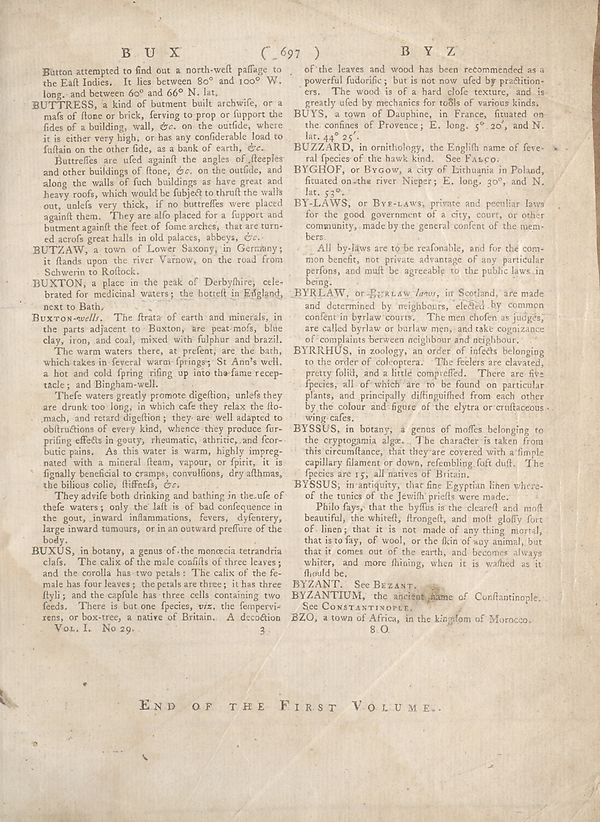
\includegraphics[width=0.85\textwidth]{../scans/page-2250-75315f455009.jpg}
\caption*{Source scan: \texttt{page-2250-75315f455009.jpg}}
\end{figure}

\end{document}
